\section{Appendices} \label{sec:appendices}
% Test programs, test data, code, etc.
\subsection{Source Code}
\subsubsection{Main Function}
\lstinputlisting[language=Haskell]{../app/Main.hs}

\subsubsection{Syntax}
\lstinputlisting[language=Haskell]{../app/Syntax.hs}

\subsubsection{Parser}
\lstinputlisting[language=Haskell]{../app/Parser.hs}

\subsubsection{Type Checker}
\lstinputlisting[language=Haskell]{../app/TypeCheckAnnotate.hs}

\subsubsection{AST Reversing}
\lstinputlisting[language=Haskell]{../app/AstReversing.hs}

\subsubsection{Evaluating Constant Expressions}
\lstinputlisting[language=Haskell]{../app/EvalExpr.hs}

\subsubsection{Optimizer}
\lstinputlisting[language=Haskell]{../app/AssertionRemoval.hs}

\subsubsection{AST Renaming}
\lstinputlisting[language=Haskell]{../app/RenameProcedures.hs}

\subsubsection{\texttt{C++} Code Generation}
\lstinputlisting[language=Haskell]{../app/JapaToCpp.hs}

\subsubsection{Running tests}
\lstinputlisting[language=bash]{../bin/tester.sh}
\begin{figure}
    \centering
    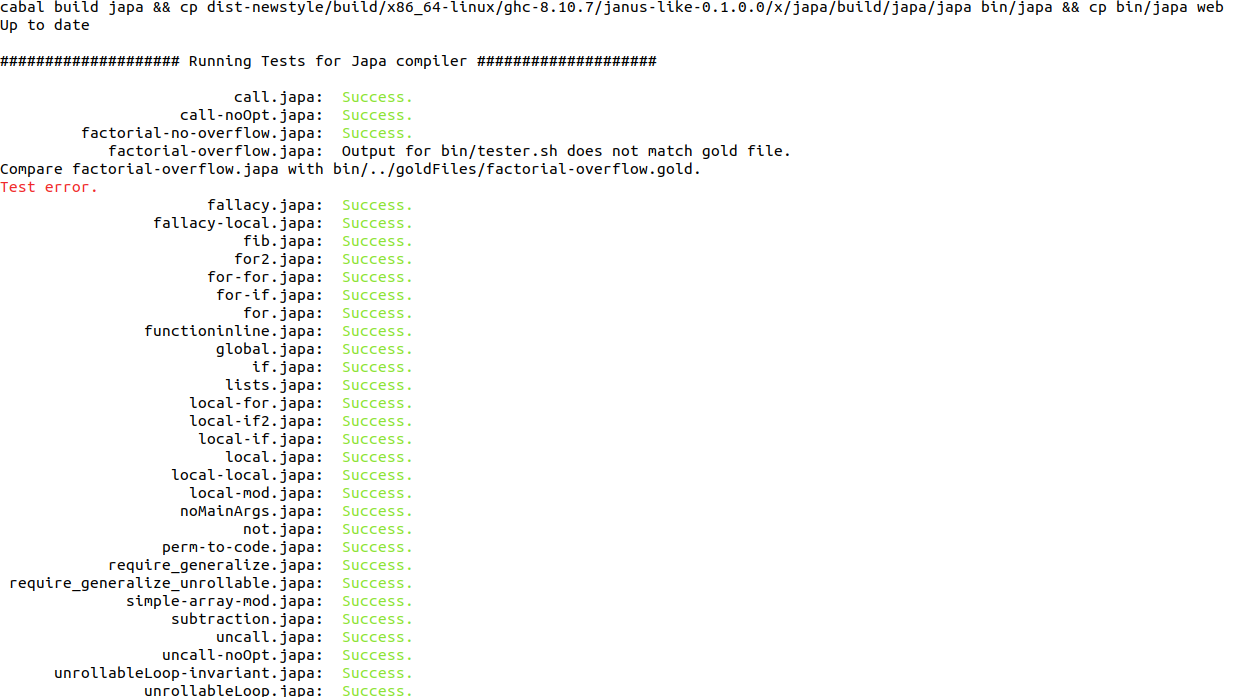
\includegraphics{imgs/testrun.png}
    \caption{A run through of the different gold file tests.}
    \label{fig:testrun}
\end{figure}

\subsubsection{Makefile}
\lstinputlisting[language=bash]{../Makefile}

\subsubsection{Benchmark script}
\lstinputlisting[language=Bash, label={lst:runbenchmark}]{../benchmarks/runbenchmark.sh}

\subsubsection{Benchmark programs} \label{sec:benchmark-programs}
\lstinputlisting[language=c++]{../web/examples/factorial.japa}
\lstinputlisting[language=c++]{../web/examples/fib.japa}
\lstinputlisting[language=c++]{../web/examples/perm-to-code.japa}
\lstinputlisting[language=c++]{../web/examples/unrollableLoop-invariant.japa}